\section{Versionskontrolle}
\subsection{Versionskontrollsysteme (VCS)}

\begin{multicols}{2}
	\subsubsection{Zweck}
	\begin{itemize}
		\item Aufbewahrung, Verwaltung, Wiederherstellen von Dateien \newline in einem Archiv
		\item Koordination des Zugriffs
	\end{itemize}
	
	\subsubsection{Einsatz}
	\begin{itemize}
		\item Softwareentwicklung
		\item Content-Management-Systeme (CMS)
		\item Archiv $=$ Repository $=$ Lager
	\end{itemize}
\end{multicols}

\subsubsection{Einteilung}
	\begin{itemize}
		\item Lokale Versionskontrollsysteme (LVCS), ein Archiv für jede Datei
		\item Zentralisierte Versionskontrollsysteme (CVCS), ein Archiv für alles
		\item Verteilte Versionskontrollsysteme (DVCS), mehrere verteilte Archive
\end{itemize}

\subsection{Git}
\begin{minipage}{7cm}
\begin{itemize}
	\item Git $\rightarrow$ Blödmann
	\item Entwicklet von Linus Torvalds, Linux-Erfinder
	\item Man arbeitet mittels einer Konsole, kein GUI
	\item Git ist ein DVCS
\end{itemize}
\end{minipage}
%\hfill
\begin{minipage}{9cm}
	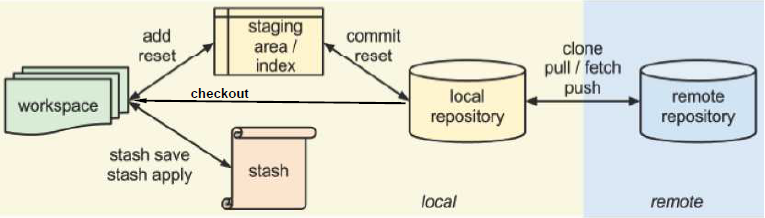
\includegraphics[width=11cm]{images/git.png}
\end{minipage}

\subsubsection{Allgemeines}
\begin{tabular}{|l|l|}
	\hline \textbf{Repository} &
    Ist ein Archiv für ein Projekt und enthält alle Änderungen und Versionen
    \\ 	\hline     
    \textbf{Branch} &
    Beschreibt zusammenhängende Änderungen in einem Projekt. Es gibt Minimum einen  bis beliebig viele.
    \\
    &
    Der Master-Branch ist der Produktivzweig
    \\ \hline
    \textbf{Commit} &
    Beschreibt eine Änderung in einem Branch an einer Datei mit Änderungsinformation
    \\ \hline
    \textbf{Snapshot} &
    Momentanes Zeitabbild des Projektes
    \\ \hline
    \textbf{Merge} &
    Zusammenführen von Änderungen aus zwei Branches
    \\	\hline
    \textbf{Stagen} &
    Datei zum Index hinzufügen
    \\\hline
\end{tabular}
\\
\\
\begin{tabular}{|c|c|}
	\hline \textbf{Lifecycle von Dateien} & \textbf{Branch}\\
	\hline \tabbild[width=9cm]{images/git_lifecycle.png} & \tabbild[width=9cm]{images/git_branch.png}\\
	\hline
\end{tabular}

\subsubsection{Datenbereiche}
\begin{tabular}{|l|l|}
	\hline
	\begin{tabular}[c]{@{}l@{}}\textbf{Workspace}\\ -Projektverzeichniss\\ -hier wird gearbeitet\end{tabular}   & \begin{tabular}[c]{@{}l@{}}\textbf{Repository}\\ -Versionsgeschichte in Form von Commits (Revision)\\ -lokal/remote\end{tabular}   \\ \hline
	\begin{tabular}[c]{@{}l@{}}\textbf{Stash}\\ -Lager\\ -temporäres Speichern der Workspace-Daten\end{tabular} & \begin{tabular}[c]{@{}l@{}}\textbf{Staging Area/Index/Cache}\\ -sammelt Änderungen für Commits\\ -Bereitstellungsraum\end{tabular} \\ \hline
\end{tabular}

\subsubsection{Git-Konzepte}
\begin{itemize}
	\item Git-Workspace ist ein Verzeichnis welches die zu bearbeitenden Dateien eines Projektes enthält
	\item In diesem Verzeichnis ist ein Unterverzeichnis \textit{".git"}
	\item Dieses Unterverzeichnis \textit{".git"} bildet das lokale Repository
	\item Im Branch zeigen die Pointer immer auf den vorhergehenden Commit
	\item Jeder Commit bekommt einen speziellen Hashwert
\end{itemize}

\subsubsection{Git Commands}
\begin{longtable}{| p{.30\textwidth} | p{.70\textwidth} |}
	\hline 
	\textbf{Create}&
	\\ \hline
	
	git init <directory>&
	Create empty Git repo in specified directory.\newline
	Run with no arguments to initialize the current directory as a git repository.
	\\ \hline 
	
	git clone <repo>& 
	Clone repo located at <repo> onto local machine.\newline
	Original repo can be located on the local filesystem or on a remote machine
	\\ \hline  \hline
	
	\textbf{Local Changes}&
	\\ \hline 
	
	\hline 
	git status&
	List which files are staged, unstaged, and untracked  
	\\ \hline
	
	git diff& 
	Show unstaged changes between your index and working
	directory 
	\\ \hline 
	
	git diff HEAD&
	Show difference between working directory and last commit.
	\\ \hline
	
	git add <directory>&
	Stage all changes in <directory> for the next commit. Replace <directory>
	with a <file> to change a specific file or witch <.> to Stage all.
	\\ \hline 
	
	git commit -m " \" <message>"&
	Commit the staged snapshot, but instead of launching a text editor, use
	<message> as the commit message.
	\\ \hline
	
	git commit -a&
	Commit all local changes in tracked files.  
	\\ \hline 
	
	gitt commit --amend&
	Change the last commit. \textbf{Don‘t amend published commits!}
	\\ \hline \hline
	
	\textbf{Commit History}&  
	\\ \hline 
	
	\hline
	git log&
	Display the entire commit history using the default format.
	\\ \hline 
	
	git log -p <file>&
	Show changes over time for a specific file 
	\\ \hline
	
	git log --author="\"<pattern>"&
	Search for commits by a particular author. 
	\\ \hline
	
	git blame <file>& 
	Who changed what and when in <file>
	\\ \hline \hline
	
	\textbf{Branches and Tags}&  
	\\ \hline
	
	\hline
	git branch&
	List all of the branches in your repo. Add a <branch> argument to
	create a new branch with the name <branch>.
	\\ \hline 
	
	git branch <new-branch>&
	Create a new branch based
	on your current HEAD
	\\ \hline
	
	git branch -d <branch>&
	Delete a local branch
	\\ \hline   
	
	git branch -dr <remote/branch>&
	Delete a branch on the remote
	\\ \hline
	
	git checkout -b <branch>&
	Create and check out a new branch named <branch>. Drop the -b
	flag to checkout an existing branch.
	\\ \hline 
	
	git merge <branch>&
	Merge <branch> into the current branch.
	\\ \hline
	
	git tag <tag-name>&
	Mark the current commit with a tag (v1.0.1)
	\\ \hline  \hline
	
	\textbf{Update and Publish}&
	\\\hline 
	
	\hline
	git remote -v&
	List all currently configured remotes.
	\\ \hline 
	
	git remote add <name> <url>& 
	Add new remote repository, named <remote>
	\\ \hline 
	
	git fetch <remote>&  
	Download all changes from <remote>,
	but don‘t integrate into HEAD
	\\ \hline
	
	git pull <remote> <branch>&
	Download changes and directly merge/integrate into HEAD  
	\\ \hline 
	
	git push <remote> <branch>&
	Publish local changes on a remote
	\\ \hline \hline
	
	\textbf{ Merge and Rebase}&
	\\\hline 
	
	\hline
	git merge <branch>&
	Merge <branch> into your current HEAD
	\\ \hline 
	
	git rebase <branch>& 
	Rebase your current HEAD onto <branch>!\textbf{Don‘t rebase published commits!}
	\\ \hline 
	
	git rebase --abort&
	Abort a rebase
	\\ \hline 
	
	git mergetool& 
	Use your configured merge tool to solve conflicts
	\\ \hline \hline
	
	\textbf{Undo}&
	\\\hline 
	
	\hline
	git reset --hard HEAD&
	Discard all local changes in your working directory.
	\\ \hline  
	
	git checkout HEAD <file>&
	Discard local changes in a specific file
	\\ \hline   
	
	git revert <commit>&
	Revert a commit (by producing a new commit with contrary changes)
	\\ \hline    
	
	git reset <commit>&
	Move the current branch tip backward to <commit>, reset the staging area to match, but leave the working directory alone. 
	\\ \hline
\end{longtable}

\subsubsection{Bashprints}
\begin{multicols}{2}
	\begin{minipage}[l]{.40\textwidth}
		Files changed but not staged.\\    
		\textbf{\$ git status}\\
		On branch master\\
		Your branch is up-to-date with 'origin/master'.\\
		Changes not staged for commit:\\
		\quad (use "git add <file>..." to update what will be committed)\\
		\quad (use "git checkout -- <file>..." to discard changes in working directory)\\
		\\
		\qquad modified:\quad idiotenseite/IdiotenseiteInclude.tex\\
		\\
		no changes added to commit (use "git add" and/or "git commit -a")\\
	\end{minipage}
	
	\begin{minipage}[r]{.40\textwidth}
		\textbf{\$ git log}\\
		commit 1b7ff854a491397087ff89689a535c275549e6ee\\
		Author: \quad Michel Gisler <Michel Gisler>\\
		Date:  \quad  Tue May 31 15:08:58 2016 +0200\\
		\\  
		\qquad Kleiner Ergänzungen und Anpasungen\\
	\end{minipage}
\end{multicols}